\chapter{Propiedades térmicas reticulares} \label{Ch:05}

En este Tema se estudia la parte más \textit{física} de las vibraciones atómicas en los sólidos. En concreto, veremos cómo se pueden entender desde la dinámica de red propiedades como \textit{calor específico}, la \textit{conductividad térmica} y la \textit{dilatación térmica} de los sólidos.

\section{Densidad de modos}

\subsection{Condiciones de contorno}

Se trata de incluir cuantitativamente el hecho de que todo cristal es finito. Sea un cristal de dimensiones $N_i \an_i  \ (i=1,2,3)$ siendo los $\an_i$ ejes primitivos $N=N_1N_2N_3$ el número de celdas primitivas. Imponiendo sobre las soluciones $\un(\Rn,t)= \epsilonn e^{i(\kn \cdot \Rn - \omega t)}$ las llamadas \textbf{condiciones de contorno periódicas} o \textbf{condiciones de contorno de Born-von Karman}, $\un(\Rn + N_i \an_i) = \un (\Rn)$ para cualquier $i=1,2,3$ se encuentra que los vectores $\kn$ son de la forma

\begin{equation}
	\kn = \frac{n_1}{N_1} \bn_1 + \frac{n_2}{N_2} \bn_2 + \frac{n_3}{N_3} \bn_3 \ \text{con} \ \an_i \bn_j = 2 \pi \delta_{ij} \label{Ec:05-01-01}
\end{equation}
donde los $n_i$ son, en principio, cualquier entero. Hemos visto sin embargo que sólo hay que considerar los vectores de onda dentro de la $PZB$. Es fácil de ver que en cualquier celda primitiva de la red recíproca, por ejemplo en la $PZB$, sólo existen, según (\ref{Ec:05-01-01}), $N_1N_2N_3=N$ \textit{valores de $\kn$ posibles}. Por lo visto del tema \ref{Ch:04}, existirán un total de $3zN$ modos normales. El volumen asociado a cada valor permitido de $\kn$ es $V_{PZB}/N$. Como el volumen total del cristal se puede escribir como $V=V_{\text{celda}} N$ y $V_{\text{celda}} = 8 \pi^3 /V_{PZB}$, resulta que el volumen asociado a cada valor de $\kn$ es $8 \pi^3/ V$.

\begin{figure}[h!] \centering
    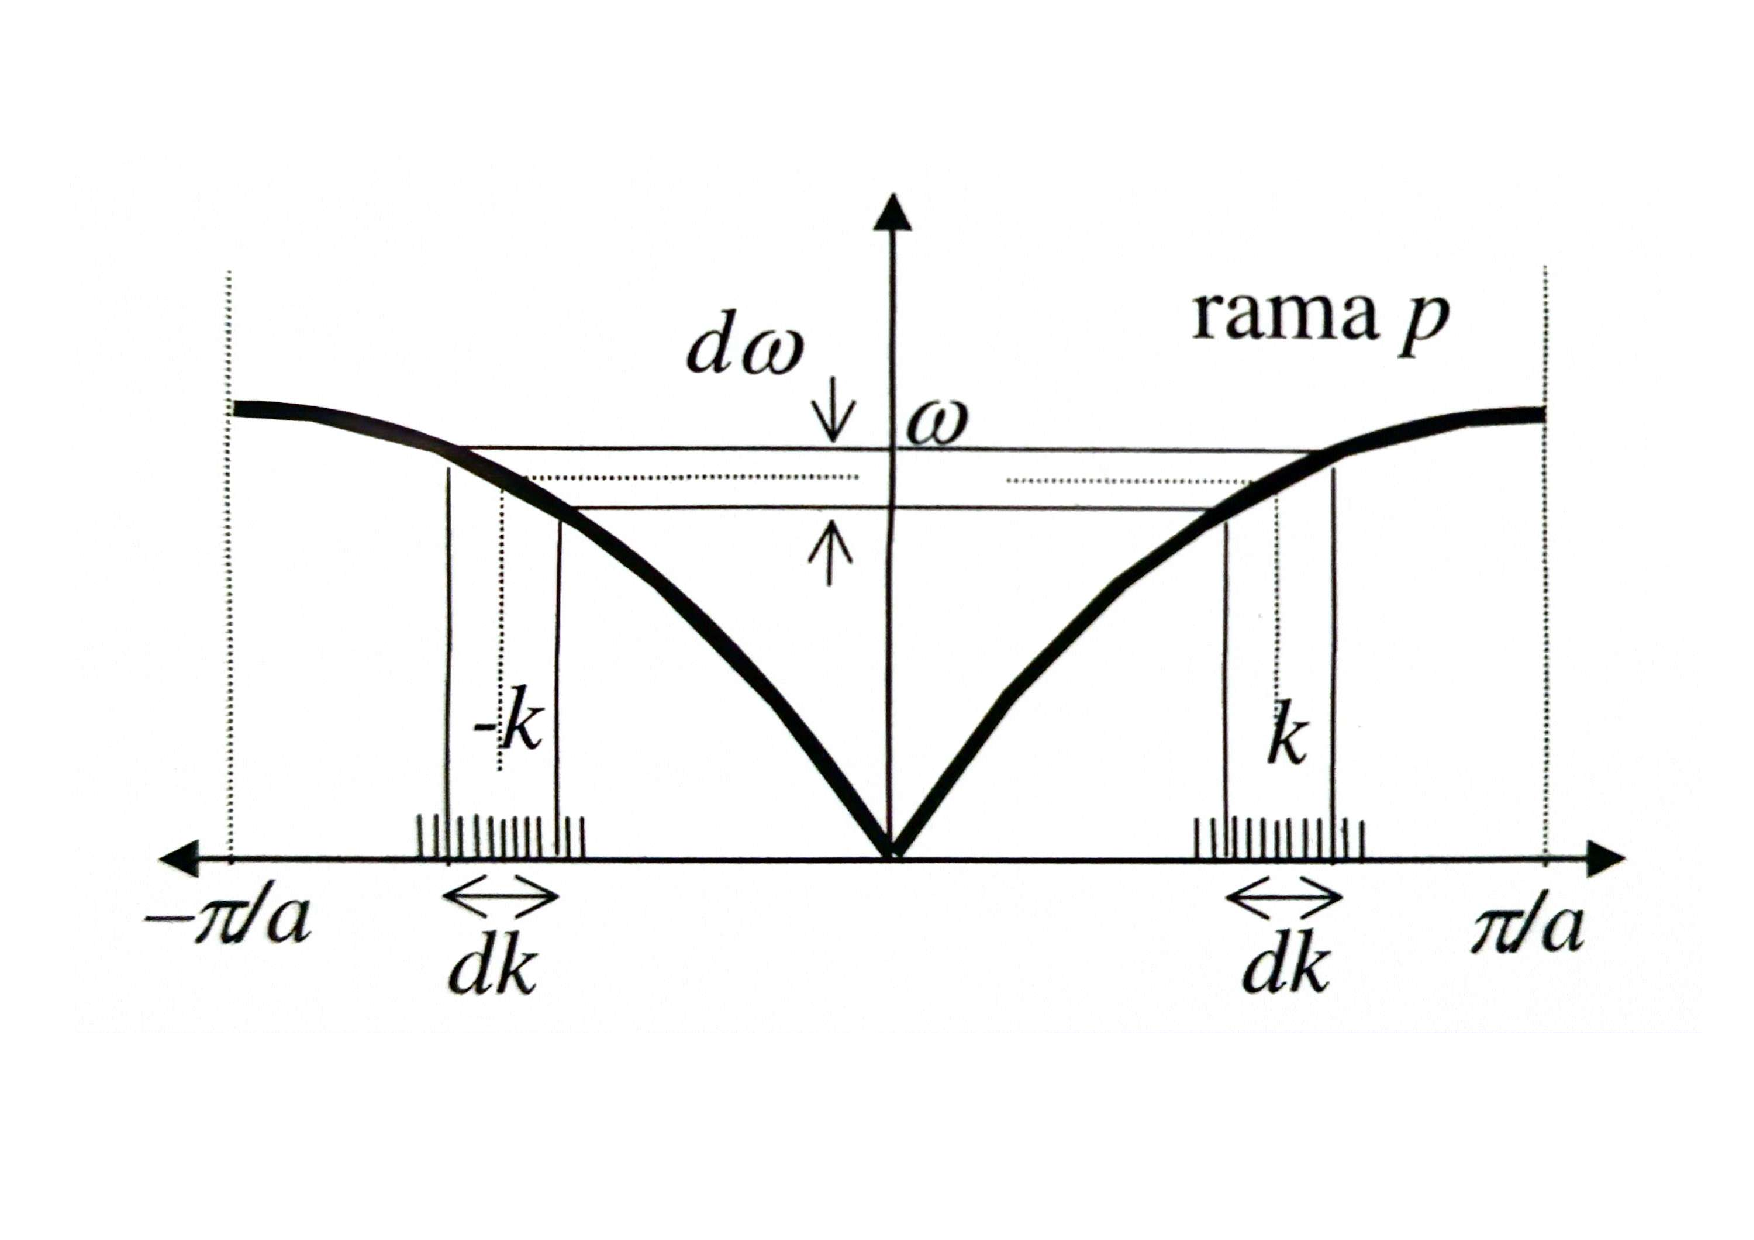
\includegraphics[scale=0.36]{Cuerpo/Ch_05/Fotos libro 1.pdf}
    \caption{Relación de dispersión para una cadena monoatómica. Equivalencia entre la densidad de modos en $k$ y en $\omega$.}
    \label{Fig:05-01}
\end{figure}    


\subsection{Cálculo de la densidad de modos}

Para el estudio de muchas propiedades cristalinas es importante conocer cómo se \textit{reparten} los modos posibles no en $\kn$ sino en frecuencia $\omega$. Se define así la \textit{densidad de modos} o \textit{estados} para la rama $p$, $D_p (\omega)$, como el número de modos por unidad de frecuencia con frecuencias en el intervalo $(\omega,\omega+\D \omega)$.

En una dimensión, si el cristal es de longitud $L=Na$, hay $N$ valores de $k$ en la $PZB$ ($-\pi/a < k\leq \pi/a$) de manera que, el intervalo $\delta k$ asociado a cada modo es $2 \pi / L$. El número de modos de una rama denotada por $p$ en el intervalo $\D \omega$ será, según se indica en la figura \ref{Fig:05-01}:

\begin{equation*}
	D_p (\omega) \D \omega = \frac{2 \D k}{\delta k} = \frac{L}{\pi} \left| \parciales{k}{w}  \right| \D \omega = \frac{L}{\pi} \frac{\D \omega}{|\nabla_l \omega (k)|_p} \Rightarrow
\end{equation*} 

\begin{equation}
	D_p (\omega)  = \frac{L}{\pi} \frac{1}{|\nabla_ k \omega (k)|_p }
\end{equation}
La generalización a dos y tres dimensiones es, respectivamente:

\begin{eqnarray}
	\text{2D}) \  D_p (\omega) &=& \int_{L_p (\omega)} \frac{S}{4\pi^2} \frac{\D L}{|\nabla_\kn \omega(\kn)|_p} \\ 
	\text{3D}) \  D_p (\omega) &=& \int_{S_p (\omega)} \frac{V}{8\pi^2} \frac{\D L}{|\nabla_\kn \omega(\kn)|_p} \label{Ec:05-01-04}
\end{eqnarray}
donde la integral se extiende sobre la línea (en 2D) o superficie (en 3D) del espacio $\kn$ con $\omega$. Finalmente, $D(\omega)=\sum_p Dp (\omega)$.
 
\subsection{Aproximación de Debye}    

Esta aproximación consiste en sustituir todas las ramas de vibración por \textit{tres idénticas e isótropas} con relación de dispersión:

\begin{equation}
	\omega = c k \quad (0<k<k_D)
\end{equation}
siendo $c$ la velocidad del sonido en el cristal (para $k\rightarrow 0$) y $k_D$ el llamado \textbf{vector de onda de Debye}. Este se escoge de tal manera que el número total de modos sea el correcto ($3zN$). La figura \ref{Fig:05-02} ilustra como $k_D$ debe ser mayor que $k_{PZB}$ precisamente para que el número total de modos sea el adecuado. Según esta definición

\begin{equation}
	3zN = 3 \times \frac{\frac{4}{3} \pi k^3_D}{\frac{8 \pi^3}{V}} \Rightarrow k_D^3 = 6 \pi^2 n
\end{equation}
siendo $n=zN/V$ la densidad numérica de átomos. 

En esta aproximación las superficies de $\omega$ constante son esferas (la figura \ref{Fig:05-03} muestra la sección para $k_z$ de una superficie $\omega=\cte.$) La densidad de modos viene dada por $D_D(\omega) \D \omega = 3 \times 4 \pi k^2 \D k / (8\pi3 /V)$, que al utilizar (\ref{Ec:05-01-04}) permite despejar 

\begin{equation}
	D_D (\omega) = \frac{3V}{2\pi^2} \frac{\omega^2}{c^3} \tquad (0<\omega<\omega_D)
    \label{Ec:05-01-07}
\end{equation}
La frecuencia máxima $\omega_D=ck_D$ se denomina \textbf{frecuencia de Debye}. 


\begin{figure}[h!] \centering
    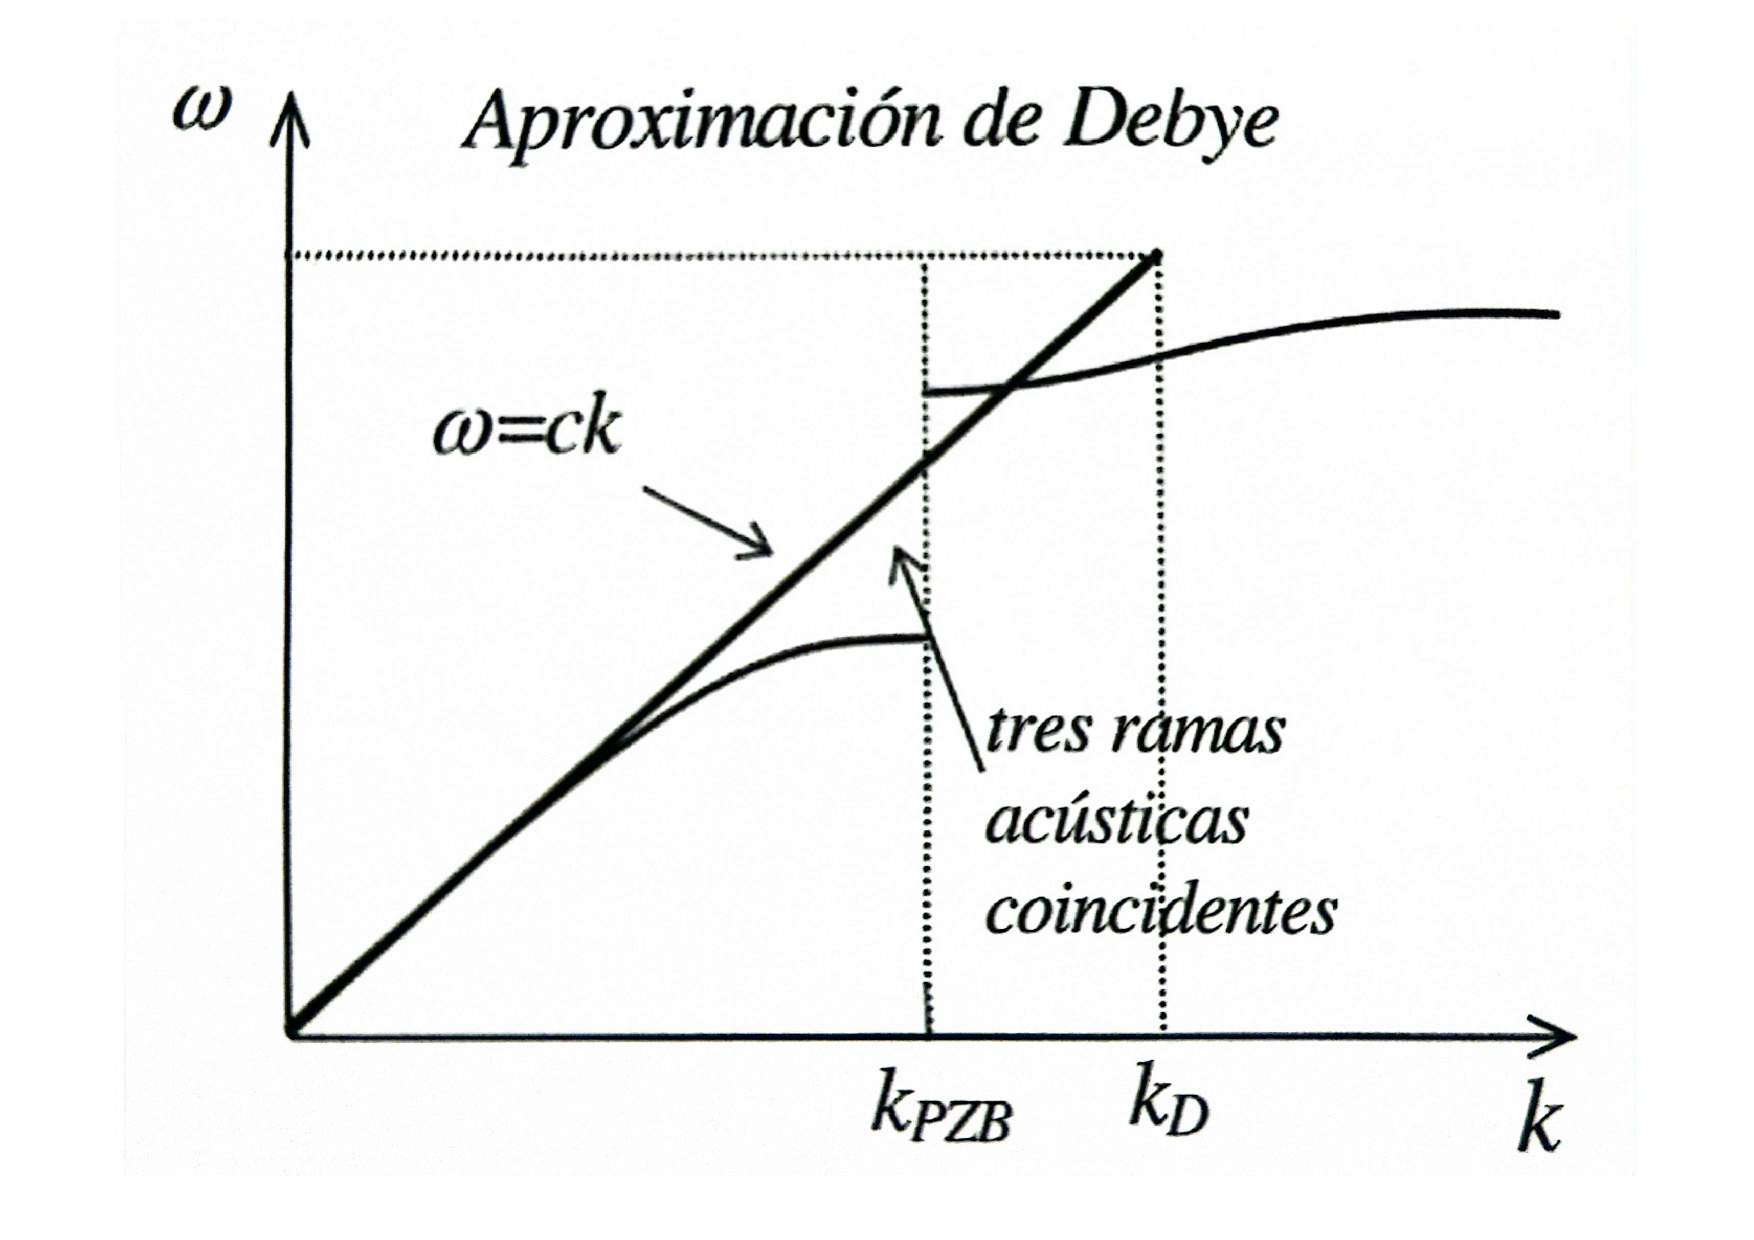
\includegraphics[scale=0.35]{Cuerpo/Ch_05/Fotos libro 2.pdf}
    \caption{Representación de la aproximación de Debye. Todas las ramas se sustituyen por tres acústicas degeneradas.}
    \label{Fig:05-02}
\end{figure}



\begin{figure}[h!] \centering
    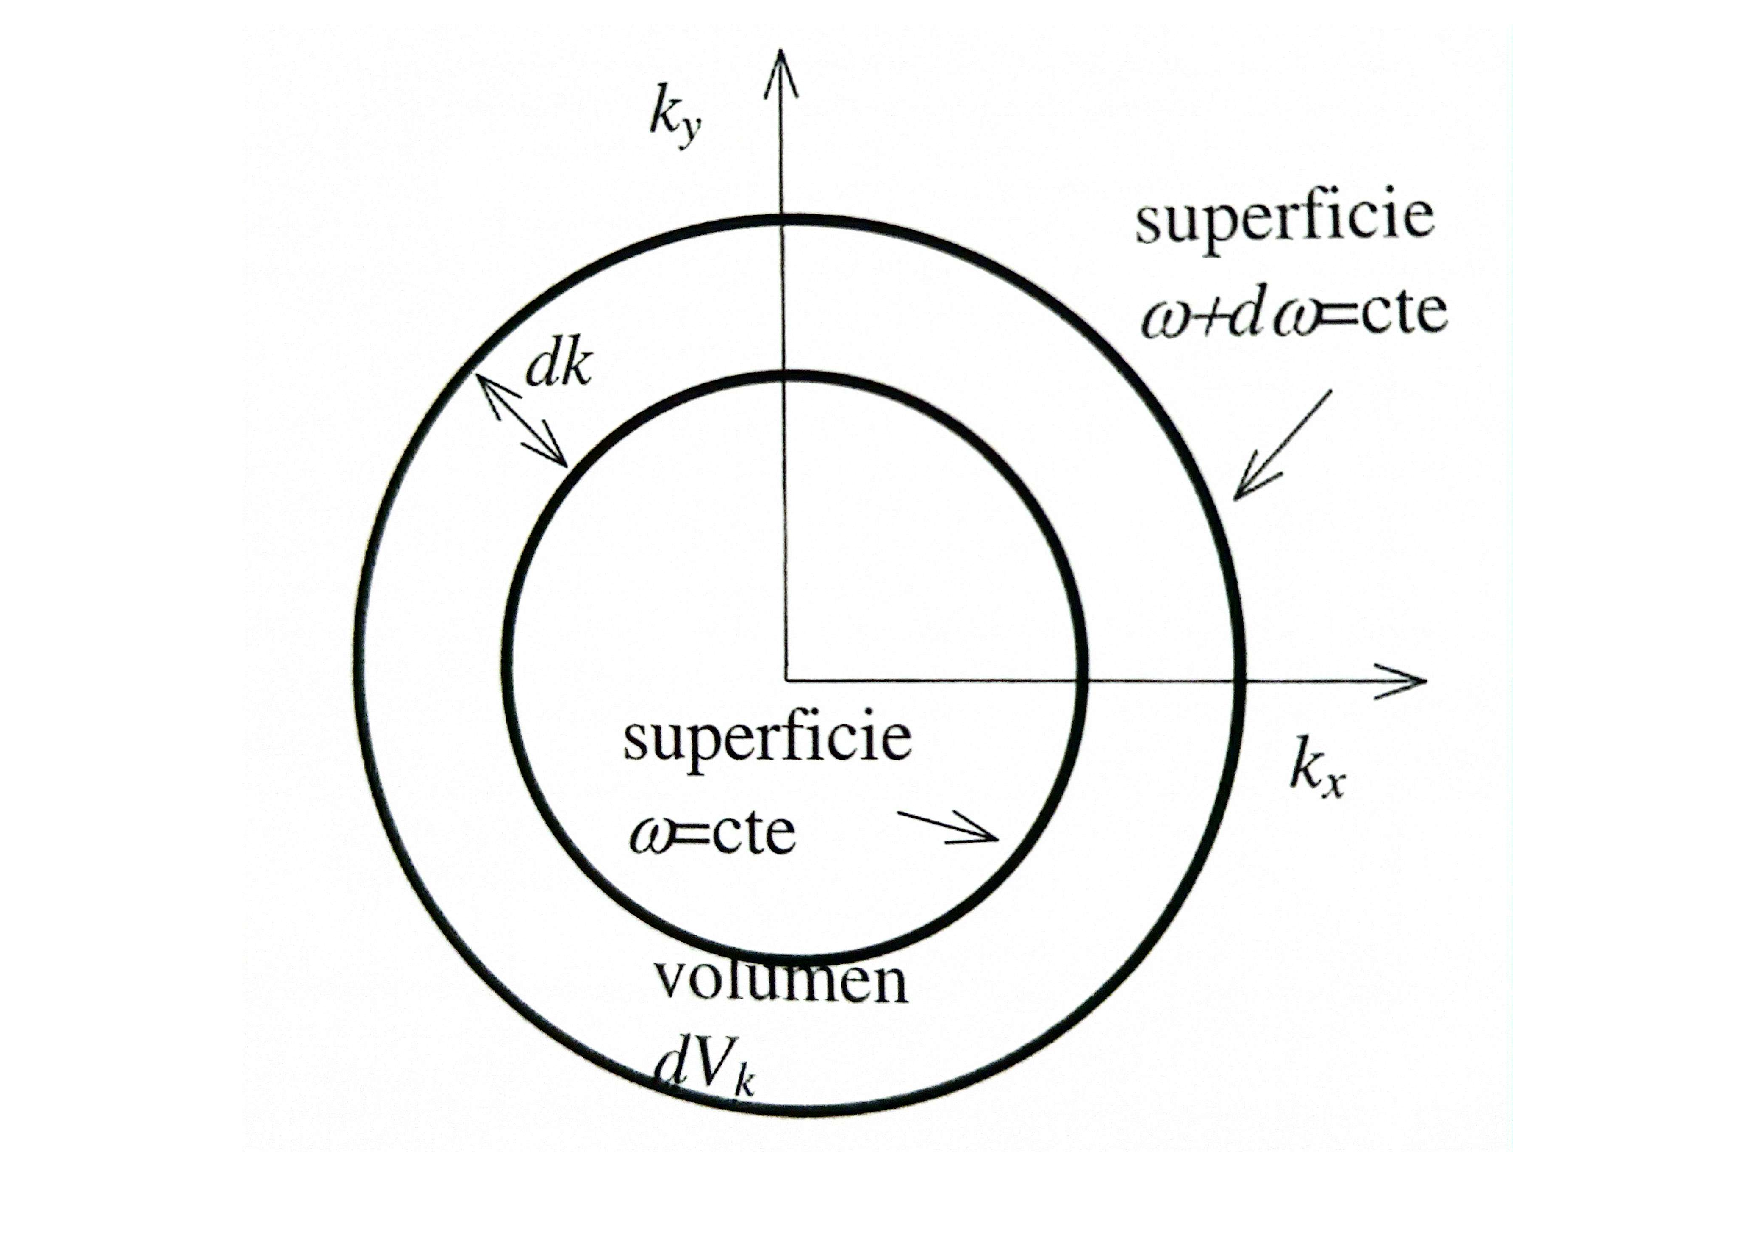
\includegraphics[scale=0.35]{Cuerpo/Ch_05/Fotos libro 3.pdf}
    \caption{Sección de una superficie de frecuencia constante en la aproximación de Debye.}
    \label{Fig:05-03}
\end{figure}    

\section{Capacidad térmica reticular}

La capacidad térmica reticular (en metales debe añadirse la asociada a los electrones por conducción) está estrechamente relacionada con la energía vibracional y por tanto con los \textit{fonones}. En concreto queremos calcular $C_V = (\partial U / \partial T)_V$. 

\subsection{Estadística de fonones}

Para determinar la energía de un modo necesitamos conocer el número medio de fonones a una temperatura $T$. El \textit{factor de Boltzmann} nos dice que la probabilidad de tener un oscilador en un estado de excitación $n$ es $P_n \propto e^{-\epsilon_n/k_B T}$ donde $\epsilon_n = (1/2+n)\hbar \omega$ es la energía del estados $n$. El número medio de excitación $\langle n \rangle$ (número medio de fonones) de un modo cualquiera $k,p$ a temperatura $T$ será:

\begin{equation}
    \langle n \rangle = \frac{\sum_{n=0}^\infty n P_n}{\sum_{n=0}^{\infty} P_n} = \frac{1}{e^{\hbar \omega/k_B T} -1}
\end{equation}
que es la conocida \textit{distribución de Plank}. La energía media del modo en cuestión será

\begin{equation}
    \langle U \rangle = \parentesis{1+\langle n \rangle} \hbar \omega
\end{equation}
Observar que a altas temperaturas $(k_B T \gg \hbar \omega)$: tenemos que

\begin{equation}
    \langle n \rangle \approx \frac{k_B T}{\hbar \omega} \Longrightarrow \langle U \rangle = k_B T
\end{equation}
que es el límtie clásico. 

\subsection{Cálculo de la capacidad térmica}

Habiendo determinado la energía media de cada modo,

\begin{equation*}
    \langle U_{\kn,p} \rangle = \parentesis{\frac{1}{2} + \langle n_{\kn,p} \rangle } \hbar \omega_p (\kn)  
\end{equation*}
la energía de la total media $U$ será la suma 

\begin{equation}
    U = \sum_{\kn,p} U_{\kn,p} = \sum_{\kn,p} \frac{\hbar \omega_p (\kn)}{e^{\hbar \omega_p (\kn)/k_B T} - 1} = \sum_p \int_{0}^{\omega_{p \max}} \frac{D_p (\omega) \hbar \omega}{e^{\hbar \omega/ k_B T} - 1} \D \omega  \label{Ec:05-02-04}
\end{equation}
donde se ha omitido la energía del punto cero por no depender de la temperatura. Se ha expresado también la suma en $\omega$ en vez de $\kn$ a través de la densidad de modos y, además debido a la alta densidad de modos, se ha sustituido la suma por una integral. La suma en (\ref{Ec:05-02-04}) se puede calcular en los casos límites aún si conocer la relación de dispersión $\omega=\omega_p (\kn)$. 

\begin{enumerate}
    \item A altas temperaturas ($k_BT \gg \hbar \omega_{\max}$) se tiene $U\approx \sum_{\kn,p} k_B T$. Como el número de modos es $3zN$, $U\approx (3zN)k_B T$, y finalmente 
    \begin{equation}
        C_V \equiv \parciales{U}{T} \approx (3zN)k_B
    \end{equation}
    Este resultado se conoce como \textbf{ley de Dulong y Petit} y expresa que el \textit{calor específico por mol} es el mismo para todos los cuerpos. 
    \item A bajas temperaturas ($k_B T \ll \hbar \omega_{\max}$) las frecuencias (\ref{Ec:05-02-04}) corresponden a la zona lineal de las ramas acústicas donde $\omega_p (\kn) \approx c_p k$, lo cual permite aproximar la función densidad de modos por $D_p (\omega) = V \omega^2 / 2 \pi^2 c_p3$. Asimismo puede aproximarse $e^{\hbar \omega_p/ k_B T} - 1 \approx e^{\hbar \omega / k_B T}$. Llamando $x=\hbar \omega / k_B T$  (\ref{Ec:05-02-04}) se puede escribir finalmente como 
    \begin{equation}
        U \approx \frac{Vk_B^4T^4}{2 \pi^2 \hbar^3} \parentesis{\sum_{p=1}^3 \frac{1}{c_p^3}} \int_0^\infty x^3 e^{-x} \D x = \frac{3Vk_B^4 T^4}{\pi^2 \hbar^3} \parentesis{\sum_{i=0}^3 \frac{1}{c_p^3}}
    \end{equation}
    Como $U\propto T^4$ se tiene que $C_V \propto T^3$, de acuerdo con lo que se observa experimentalmente. Para cristales isotrópicos $c_p=c$ para las tres direcciones espaciales ($p=1,2,3$) con lo cual
    \begin{equation}
        U \approx \frac{9V(k_B T)^4}{\pi^2 c^3} \Rightarrow C_V \approx \frac{36Vk_B^4}{\pi \hbar^3 c^3} T^3
    \end{equation}
    \item A temperaturas intermedias se necesita alguna aproximación. Una es la de Debye, que supone admitir, como ya se ha visto, un espectro lineal. Usando (\ref{Ec:05-01-07}) en (\ref{Ec:05-02-04}) se obtiene 
    \begin{equation}
        U = \frac{3V\hbar}{2 \pi^2 c^3} \int_0^{\omega_D} \frac{\omega^3}{e^{\hbar \omega/k_B T} - 1} \D \omega
    \end{equation}
    que derivada con respecto a $T$ da
    \begin{equation}
        C_V = \frac{3V\hbar}{2 \pi^2 c^3 k_B T^2} \int_0^{\omega_D} \frac{\omega^4}{\parentesis{e^{\hbar \omega/k_B T} - 1}} \D \omega
    \end{equation}
    Se define la \textbf{temperatura de Debye} $\theta_D$ por $k_B\theta_D=\hbar \omega_D$, la cual representa básicamente la temperatura a partir la cual todos los modos de vibración de un sólido están excitados, y en consecuencia, aquélla a partir de la cual empieza el \textit{comportamiento clásico}. En términos de $\theta_D$ y teniendo en cuenta que $c=\omega_D /k_D = k_B \theta_D / \hbar (6 \pi^2 z N/V)^{1/3}$, $C_V$ se puede expresar como
    \begin{equation}
        C_V = 9zNk_B \parentesis{\frac{T}{\theta_D}}^3 \int_0^{\theta_D/T} \frac{x^4 e^x}{\parentesis{e^x-1}^2}\D x \label{Ec:05-02-10}
    \end{equation}
    donde de nuevo $x=\hbar \omega / k_B T$. Esta ecuación predice que la capacidad térmica molar $C_V$ es una función universal de $T/\theta_D$ para todos los sólidos. Esto está en excelente acuerdo (dentro del 1-2\%) con los resultados experimentales que ilustramos en la figura Fig. \ref{Fig:05-04}, donde la línea continua representa la expresión (\ref{Ec:05-02-10}). Algunas temperaturas de Debye las representamos en la tabla \ref{Tab:05-01}.
\end{enumerate}

\begin{figure}[h!] \centering
    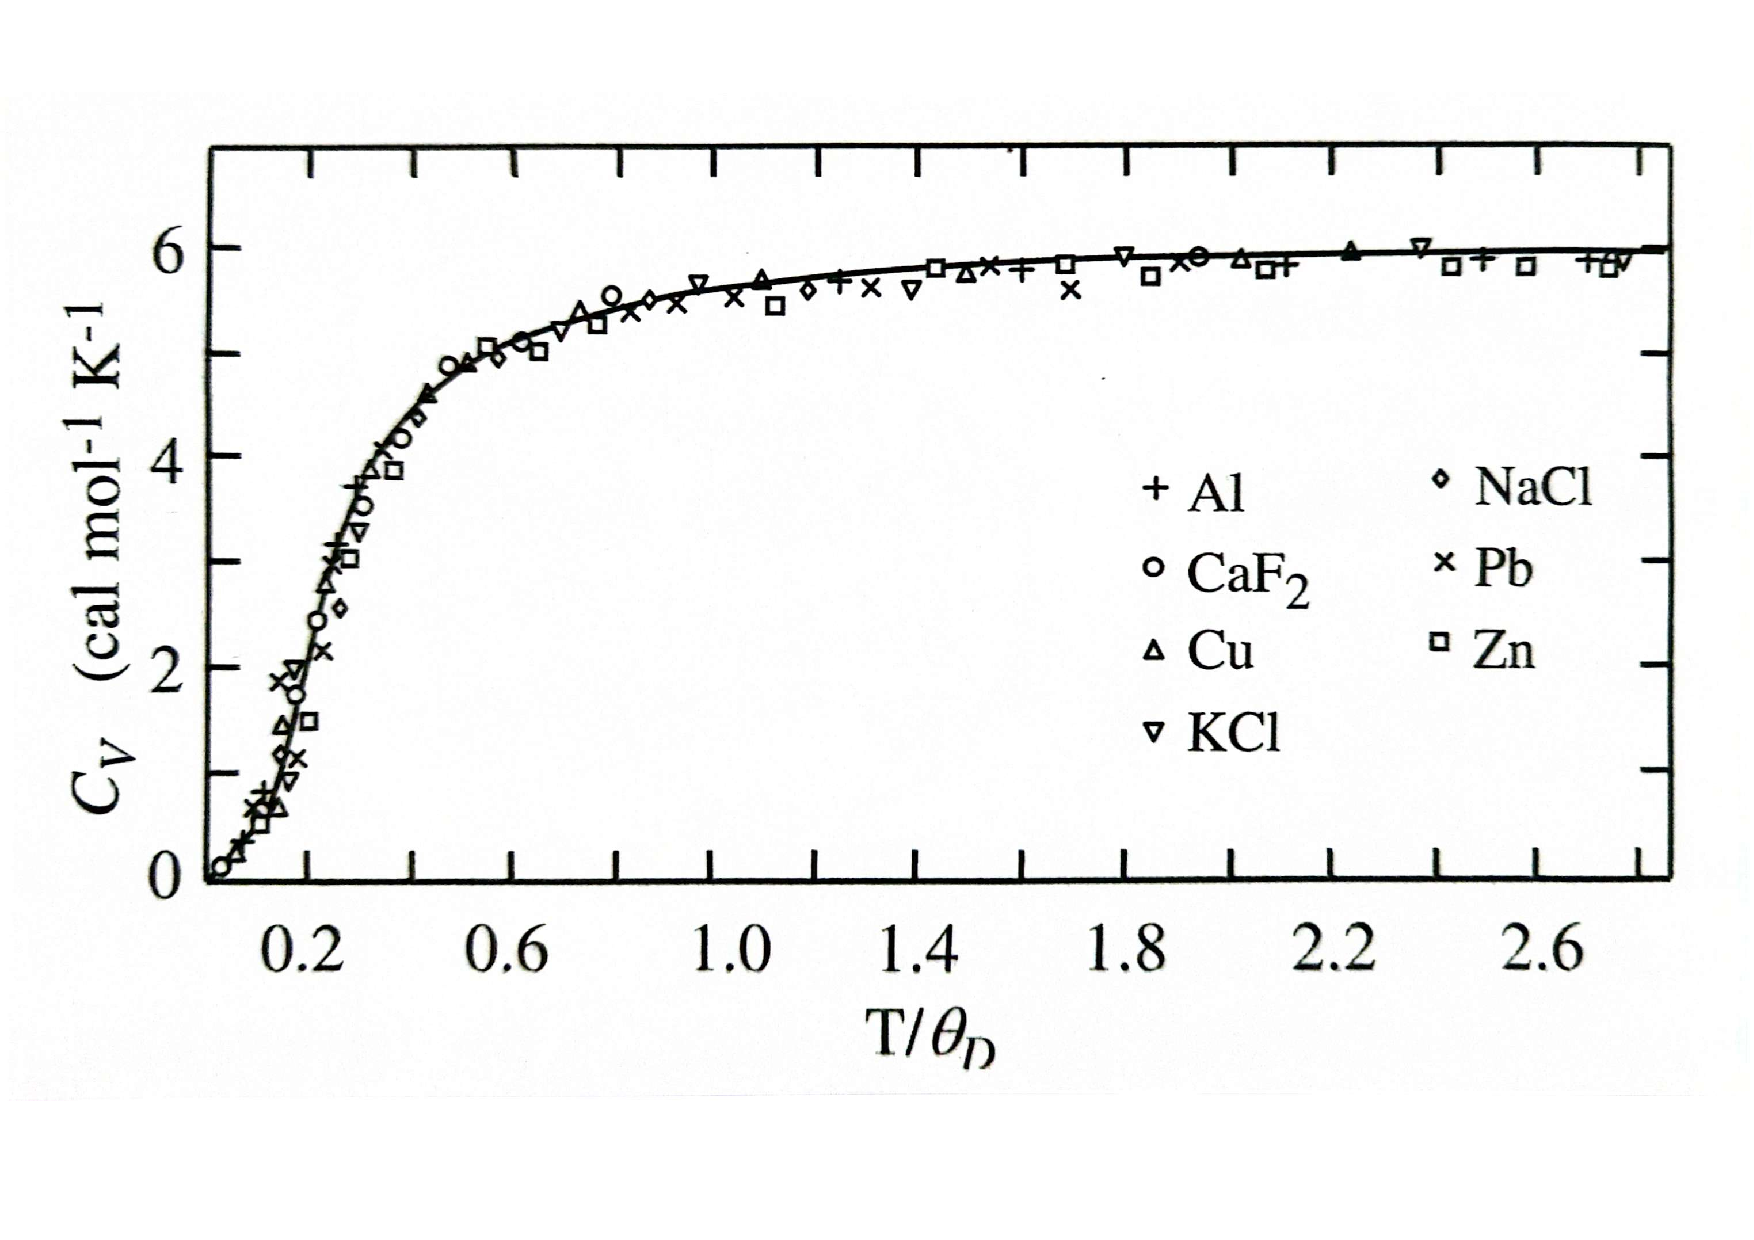
\includegraphics[scale=0.35]{Cuerpo/Ch_05/Fotos libro 4.pdf}
    \caption{Capacidad térmica por mol frente $T/\theta_D$ para diversos tipos de cristales.}
    \label{Fig:05-04}
\end{figure}    

\begin{table}[h!] \centering
\begin{tabular}{cccc}
    Elemento & $\theta_D$ ($K$) & Elemento & $\theta_D$ ($K$) \\ \hline
    Na & 158 & Ca & 230 \\
    Be & 1440 & C & 2230 \\
    Ti & 420 & Cr & 630 \\
    Fe & 470 & Ag & 225 \\
    Cu & 343 & In & 108 \\
    Pb & 105 & Bi & 119 \\
    Ar & 92 & Si & 645 \\
    Ge & 374 & Sn & 200 \\
    W & 400 & Nb & 275
\end{tabular}
\caption{temperatuas de Debye de algunos elementos.}
\label{Tab:05-01}
\end{table}

\section{Efectos anarmónicos}

Existe, como vamos a ver, algunas propiedades reiticulares cuya explicación exige ir más allá de la aproximación armónica. Es el caso de la \textit{dilatación térmica} y  \textit{conductividad térmica}.

\subsection{Dilatación térmica}

Se verá primero si la fuerza entre un átomo y sus vecinos dependiera linealmente de su desplazamiento (aproximación armónica) la dilatación no existiría. Para simplificar considérese el caso de sólo dos átomos unidos por un potencial armónico $U(r) = U_0 + c(r-r_0)^2$ donde $r$ es la interdistancia. \textit{Clásicamente}, a temperatura $T$, la probabilidad de encontrar una separación al sistema con una separación $r$ es $P(r)\propto e^{-U(r)/k_BT}$. La \textit{separación media} es entonces

\begin{equation}
    \langle r \rangle = \frac{\int_{-\infty}^{\infty} r P(r)\D r}{\int_{-\infty}^{\infty} P(r)\D r} = r_0 \label{Ec:05-03-01}
\end{equation}
\textit{independiente de la temperatura}, y por tanto no hay dilatación. La representación gráfica de este hecho se esquematiza en la figura \ref{Fig:05-05} a). 

\begin{figure}[h!] \centering
    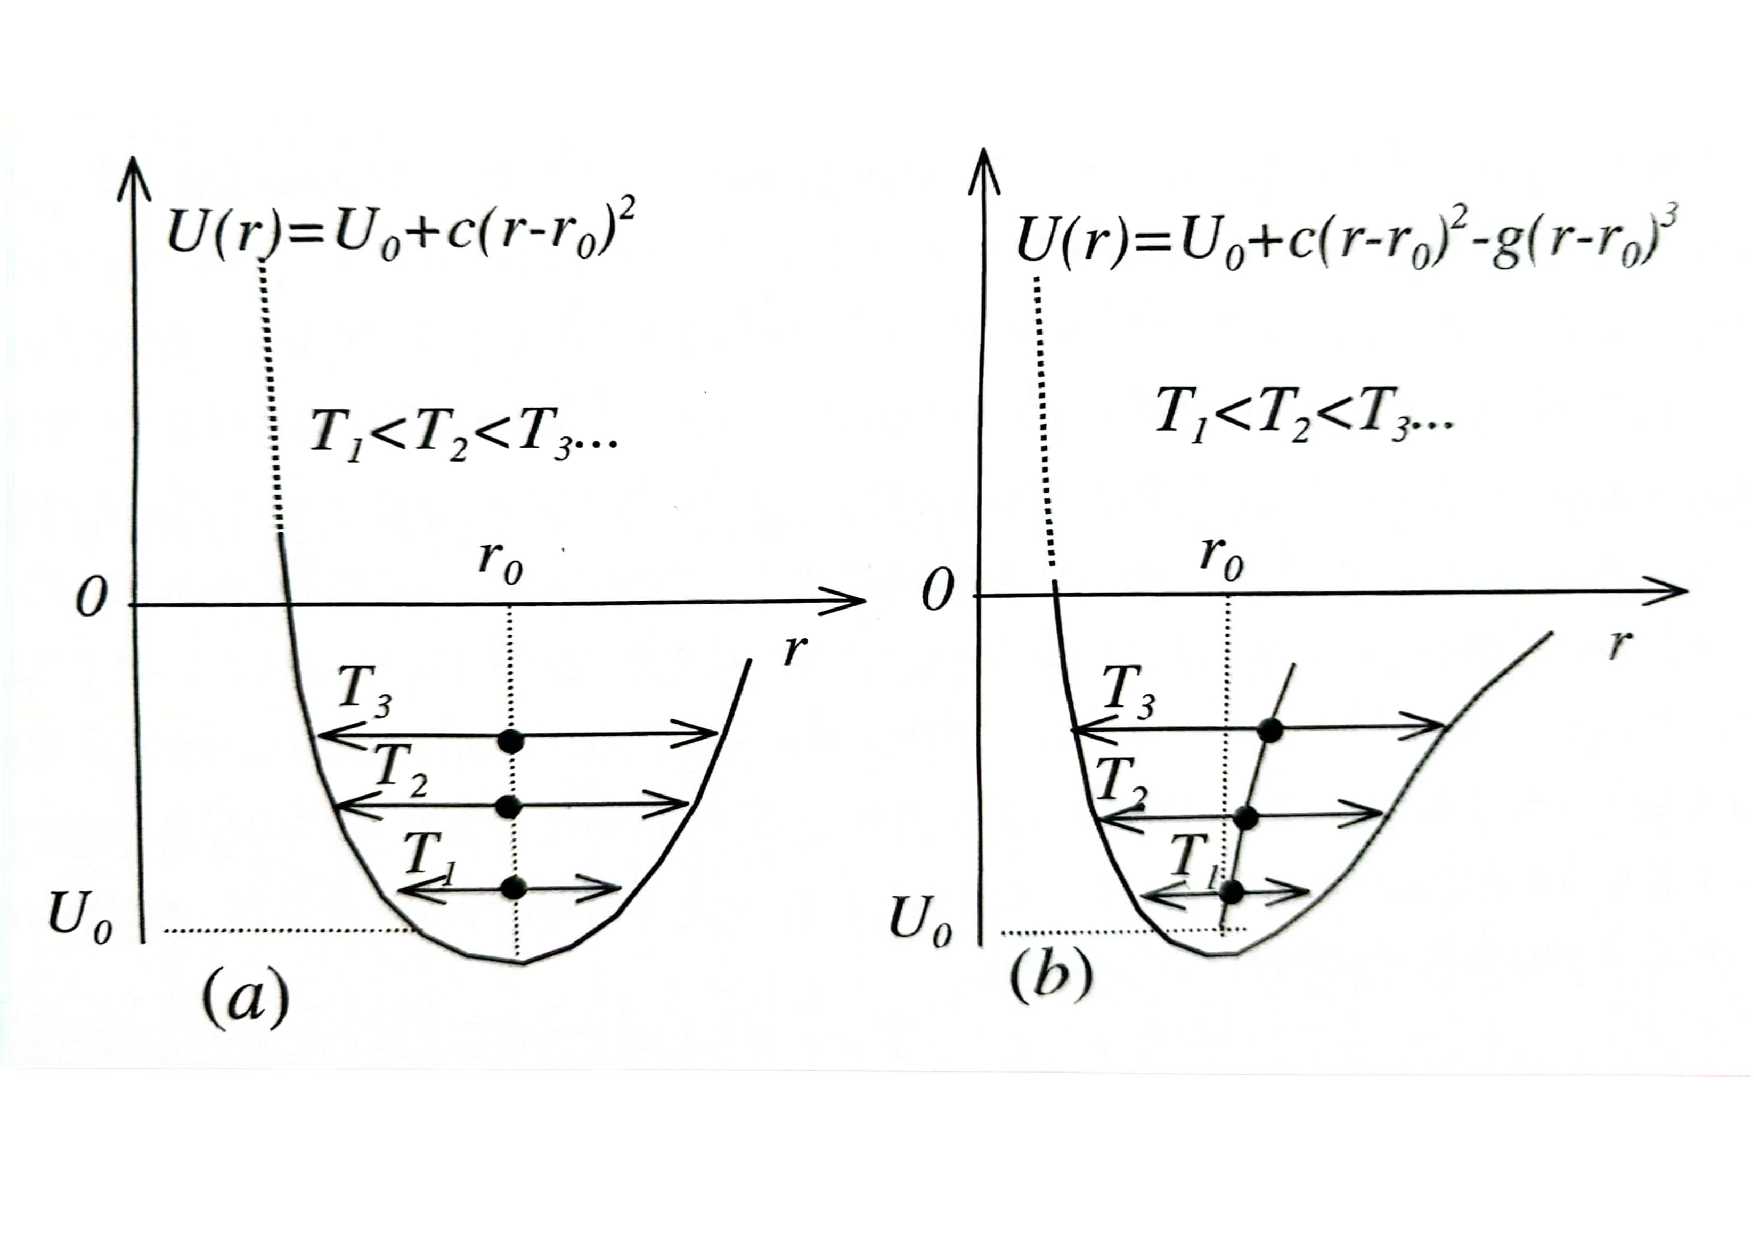
\includegraphics[scale=0.37]{Cuerpo/Ch_05/Fotos libro 5.pdf}
    \caption{Potencial por par de átomos según la aproximación armónica (a) y según la aproximación anarmónica (b) que permite explicar de los cristales cuando se calientan.}
    \label{Fig:05-05}
\end{figure}    

En segundo lugar se verá el efecto de añadir un término armónico al potencial, es decir, considerar $U(r) = U_0 + c(r-r_0)^2 - g(r-r_0)^3$. Obsérvese que $g$ tiene que ser positivo para que la contribución repulsiva decrezca más rápidamente que la distancia atractiva. La ecuación (\ref{Ec:05-03-01}) no es ahora analítica, pero si admite, que los términos armónicos son pequeños respecto a $k_BT$, puede aproximarse $e^{g(r-r_0)^3/k_BT} \approx 1 + g(r-r_0)^3 / k_BT$, en cuyo caso (\ref{Ec:05-03-01}) es resoluble, resultando en

\begin{equation}
    \langle r \rangle = r_0 + \frac{3g}{4c^2} k_B T
\end{equation}
Por tanto, la interdistancia media crece con $T$, como se muestra en la figura (\ref{Fig:05-05} (b)). Este modelo clásico predice una dilatación térmica lineal $\alpha \equiv L^{-1} (\D L / \D T)$ constante ($L$ es la longitud de la muestra), que es lo que se observa experimentalmente ($\alpha \approx 10^{-5} \unit{K^{-1}}$). Es claro que un modelo tan sencillo no considera efectos más complejos, como la anisotropía intrínseca a los sólidos cristalinos.

\subsection{Conductividad térmica}

En los sólidos la propagación del calor cumple la \textit{ley de Fourier}:

\begin{equation}
    \jn_Q = - \kappa \nabla T
\end{equation}
donde $\jn_Q$ es la densidad del \textit{flujo de calor} (W/m$^2$) y $\kappa$ es la \textit{conductividad térmica} (W/mK). En cristales $\kappa$ es en general un tensor, pero aquí prescindiremos de esa circunstancia.

Dejando de lado aparte la contribución de los \textit{electrones libres} (muy importante en metales), la propagación de calor sólo puede hacerse por las vibraciones de los átomos, es decir, por \textit{fonones} (el mismo mecanismo para la propagación del sonido). Se puede pensar entonces en un modelo cinético consistente en un \textit{gas de fonones}. En este modelo la conductividad térmica finita está asociada a con choques de los fonones que dificultan su propagación. Sin embargo, hay que justificar primero que se le puede dar carácter \textit{corpuscular} al fonón (recuérdese que el fonón es un cuanto de energía asociado al modo normal que \textit{involucra a todos los átomos} del cristal, y por ello está \textit{deslocalizado}). Para ello basta con tener en cuenta que los distintos modos pueden superponerse y formar paquetes de onda de extensión $\Delta x$ en el espacio real y $\Delta k$ en el espacio recíproco, verificando $\Delta x \Delta k \sim 1$. Una exigencia del modelo es que $\Delta k$ debe estar bien definido en el espacio recíproco, o sea $\Delta \ll k_{PZB} \sim a^{-1}$ ($a\equiv$ distancia intraatómica). Esto implica que $\Delta x$ debe ser mucho mayor que $a$. El modelo será pues aplicable siempre que las longitudes características involucradas (por ejemplo, el \textit{recorrido libre medio}, ver después) sean a su vez mucho mayores que $a$. 

\subsubsection{Cálculo de $\kappa$}

El modelo cinético que se utiliza para obtener la conductividad térmica (\textit{modelo de Drude}) está basado en las siguientes aproximaciones.

\begin{enumerate}
\item Las partículas colisionan con obstáculos con una probabilidad de colisión por unidad de tiempo $\tau^{-1}$. 
\item Entre colisión y colisión no hay interacción entre partículas: \textit{aproximación de partículas independientes}.
\item Las colisiones \textit{mantienen el equilibrio térmico local}, que quiere decir que el número de fonones en un sitio lo determina la temperatura local, y también que la velocidad con que una partícula emerge de un colisión no está relacionado con velocidad que llevaba antes de la colisión, sino que es al azar en dirección proporcional (en modulo) a la temperatura local.
\end{enumerate}

Con las anteriores aproximaciones se puede demostrar que, en cualquier instante, el tiempo transcurrido desde la última colisión (o hasta la siguiente), promediado para todas las partícula es $\tau$; es igualmente, el tiempo medio entre sucesivas colisiones, de una partícula es también $\tau$, de ahí que $\tau$ recibe el nombre de \textit{tiempo libre medio} (entre colisiones) o \textit{tiempo de relajación}.  

Se trata de hacer un balance de flujos (recuérdese que \textit{flujo}=\textit{densidad}$\times$\textit{velocidad}) desde un punto cualquiera de referencia $O$ en el seno del cristal. La densidad de energía $u=U/V$ de los fonones depende de la posición a través de la temperatura, con lo cual $u=u[T(x)]$. Esta energía contiene esencialmente el número de fonones, porque su velocidad la supondremos constante (\textit{aproximación de Debye}). El sitio en que tuvo lugar la última colisión (antes de llegar a $O$) es la que cuenta para computar la energía y el número de fonones. Los fonones recorren una distancia media (hasta llegar a $O$) de $l=c \tau$ , lo que define el \textit{recorrido libre medio} (ver figura \ref{Fig:05-06}). Estos fonones tienen una energía $u=u[T(x)]=u[T(x_0+l\cos(\theta))]$. Sumaremos pues $j_x(\theta)=c_xu(x_0+l\cos \theta)$ a todas las direcciones (puntos $P$) (nótese que, por simetría, $j_y$ y $j_z$ deben ser nulos):

\begin{equation}
    j_x = \langle j_x(\theta) \rangle_{\theta} = \frac{1}{4\pi} \int_0^{2\pi} \D \varphi \int_0^\pi j_x (\theta) \sin \theta \D \theta 
\end{equation}
Como $c_x=-c\cos (\theta)$, se tiene

\begin{equation}
    j_x = - \frac{c}{2} \int_0^\pi u (x_0 + l \cos (\theta)) \cos (\theta) \sin (\theta) \D \theta
\end{equation}
Usando la aproximación $u(x_0+l\cos \theta) \approx u(x_0) + \parciales{u}{x} l \cos(\theta)$ es inmediato obtener:

\begin{equation}
j_x = - \frac{1}{3} cl \parciales{u}{x} = \frac{1}{3} \underbrace{\parciales{u}{T}}_{c_V} \underbrace{\parentesis{-\parciales{T}{x}}}_{-\nabla T}
\end{equation}
esto es

\begin{equation}
    \kappa = \frac{1}{3} c_V cl
\end{equation}
con $c_V=C_V/V$.

\begin{figure}[h!] \centering
    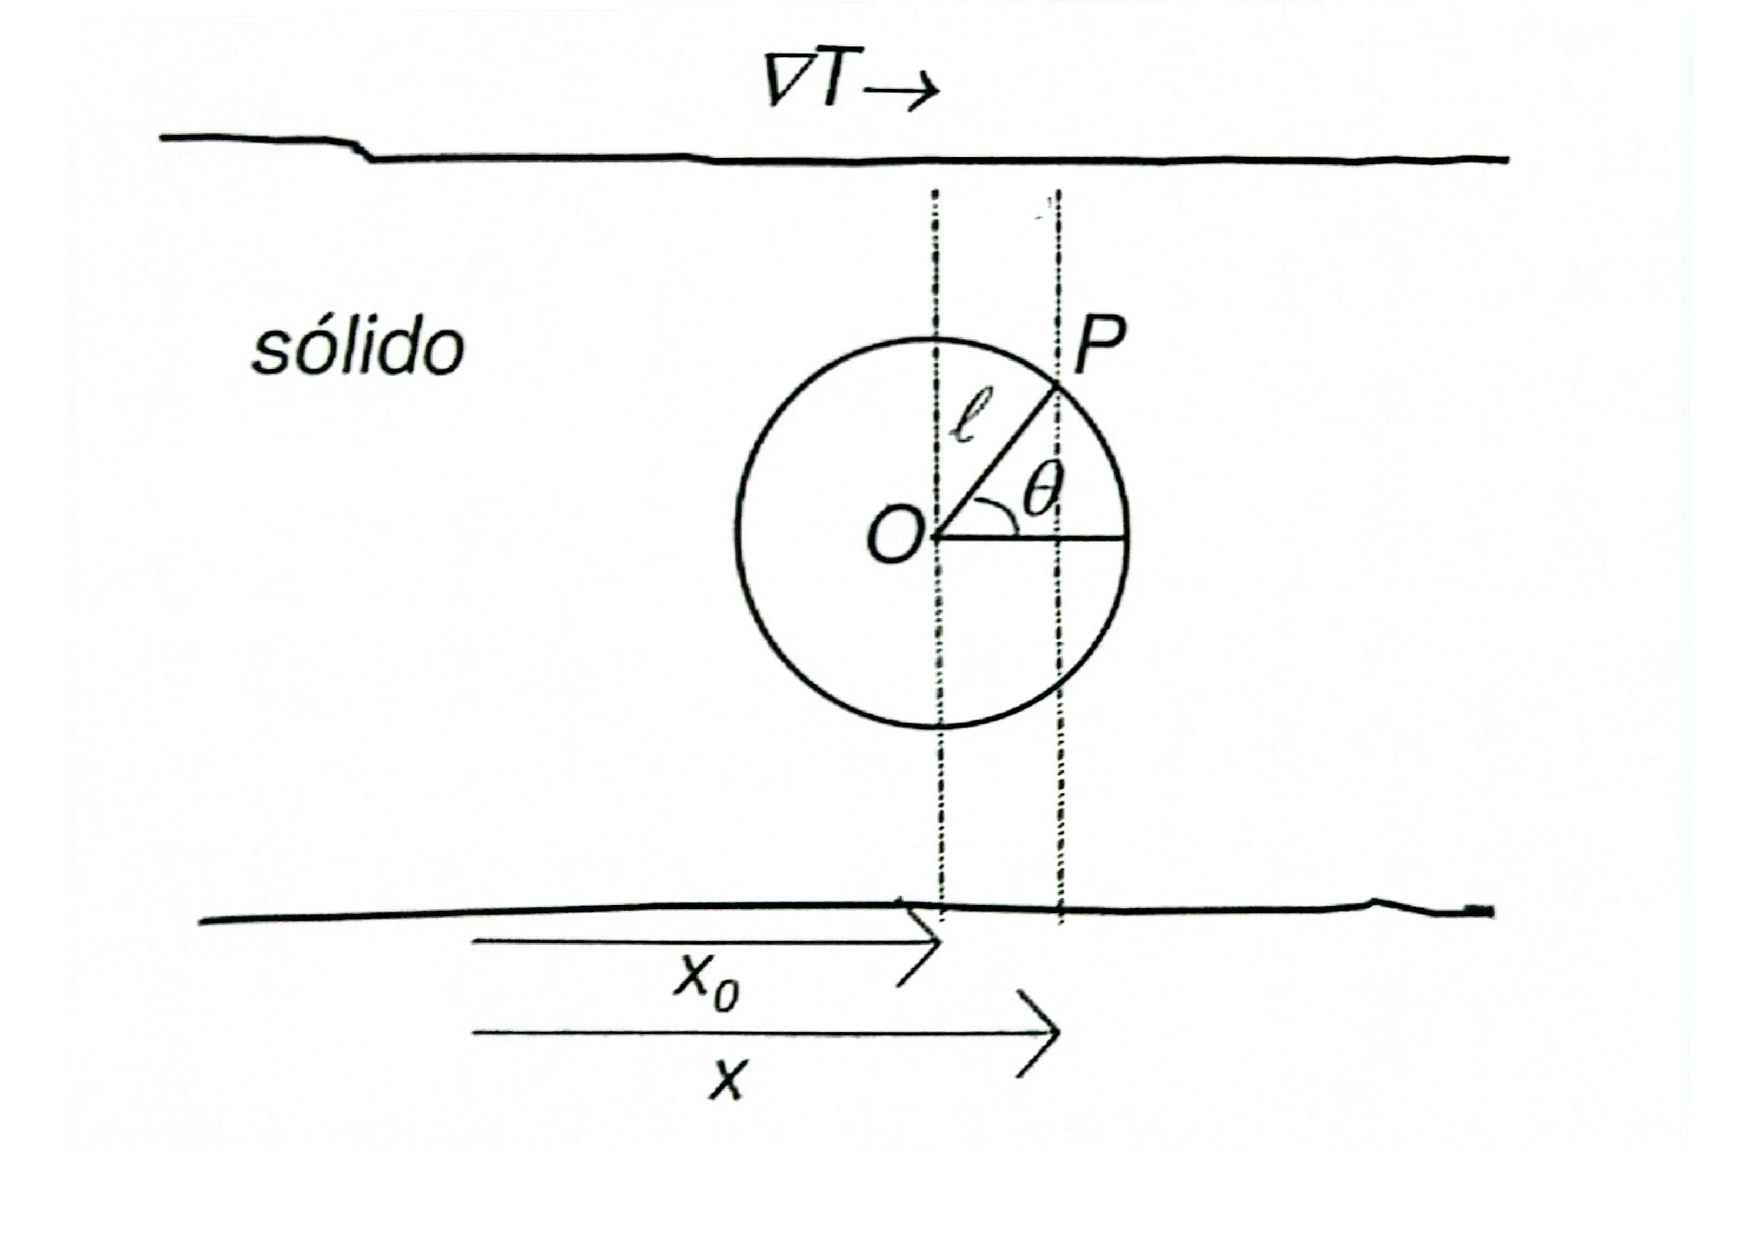
\includegraphics[scale=0.25]{Cuerpo/Ch_05/Fotos libro 6.pdf}
    \caption{Transporte de calor mediante fonones en presencia de un gradiente uniforme de temperatura. La corriente térmica en $O$ se debe a los fonones que, en media, han sufrido la última colisión en un punto $P$ a distancia $l=c\tau$.}
    \label{Fig:05-06}
\end{figure}    
 
\subsubsection{Mecanismos de \textit{scattering}}

En la aproximación armónica los modos normales son ondas elásticas que se propagan libremente sin interacción mutua. Se podría decir que los fonones tienen un recorrido libre medio infinito (es decir, no chocan). Es necesario pues introducir términos \textit{armónicos} en el potencial elástico. El lenguaje de partículas estas contribuciones dan lugar a tres fonones (figura \ref{Fig:05-07}) en las uqe se deben cumplir la conservación de la energía y del cuasiimpulso:

\begin{equation*}
    \sum \hbar \omega_i = \sum \hbar \omega_f  \tquad (i=\text{inicial}, f= \text{final})
\end{equation*}
\begin{equation}
    \sum \hbar \kn_i = \sum \hbar \kn_f + \hbar \Gn
\end{equation}

\begin{figure}[h!] \centering
    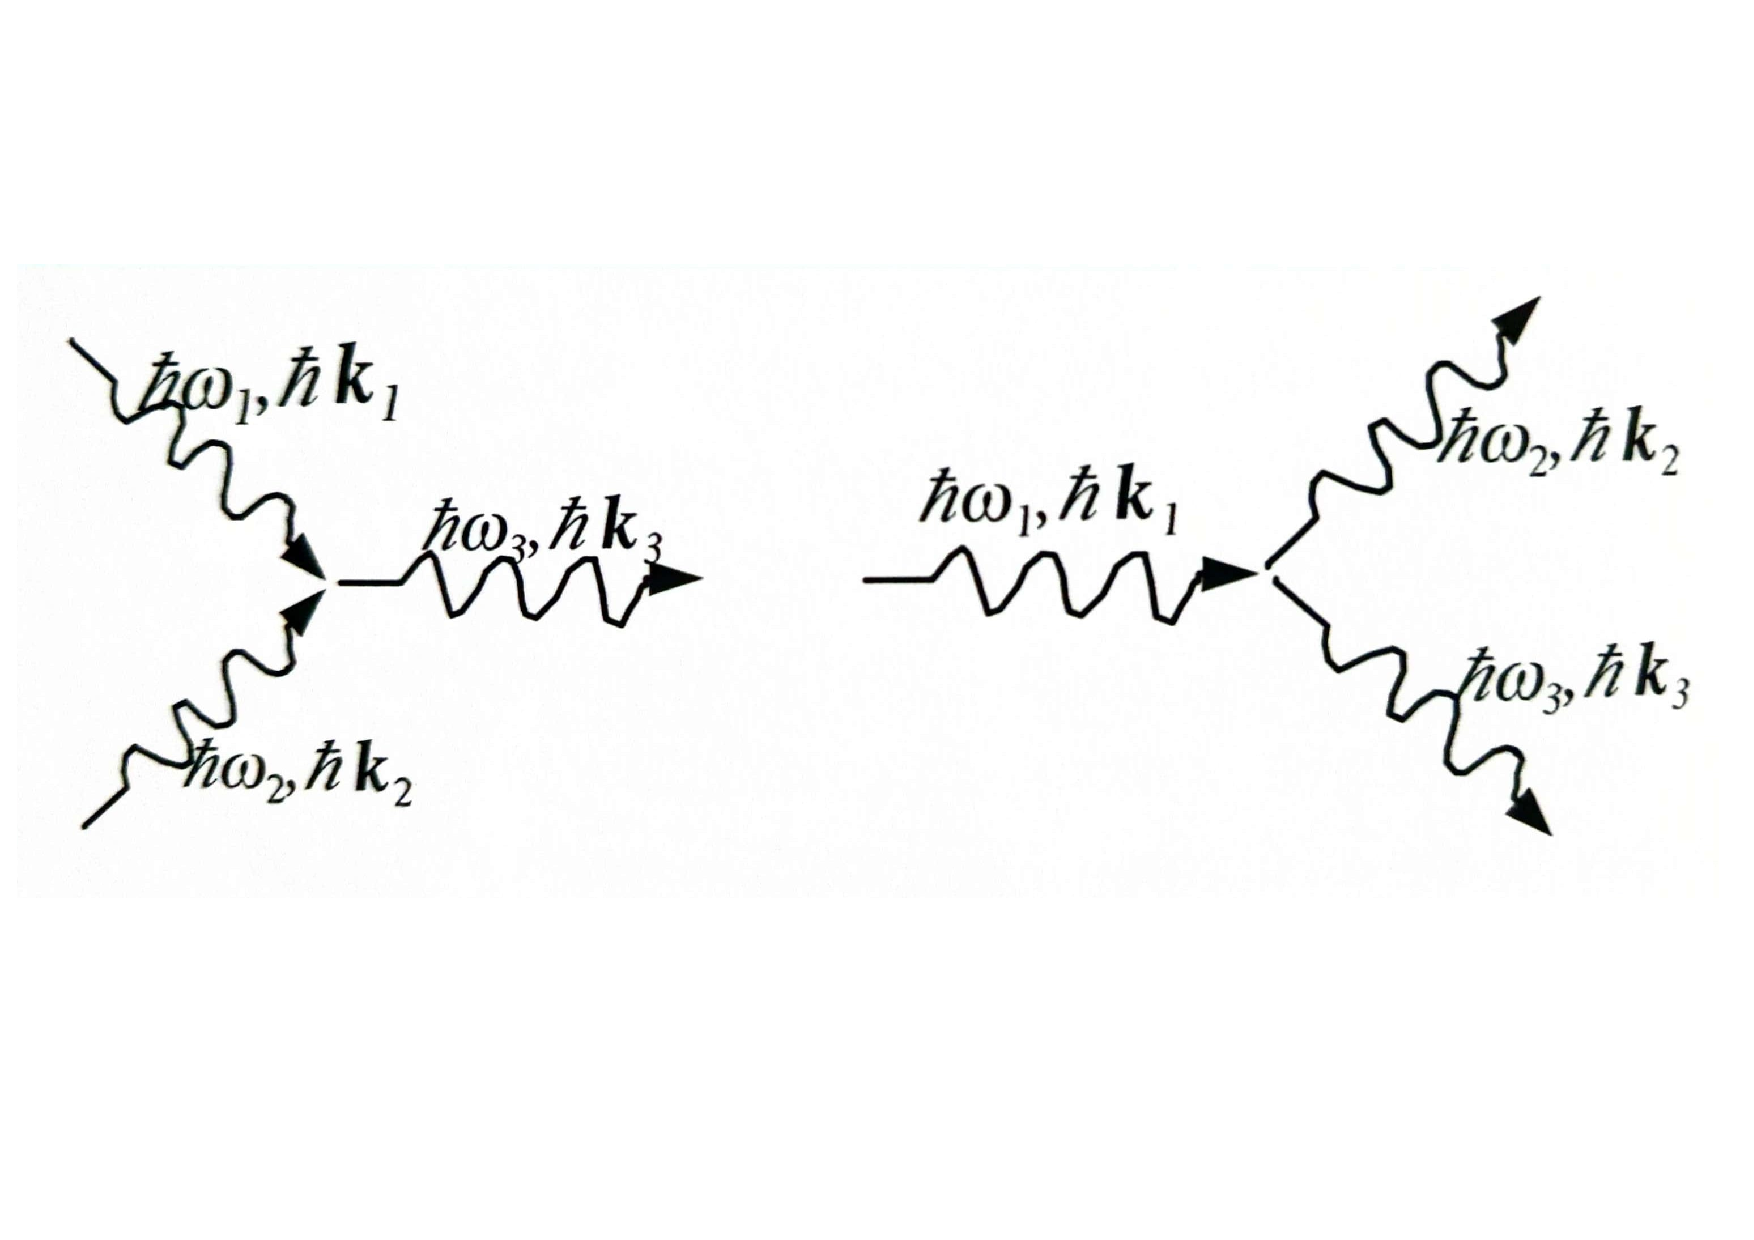
\includegraphics[scale=0.3]{Cuerpo/Ch_05/Fotos libro 7.pdf}
    \caption{Procesos de interacción entre fonones debidos a los términos (\textit{cúbicos}) anarmónicos del potencial de interacción entre átomos. Izquierda: Dos fonones interaccionan dando lugar a un tercer fonón. Derecha: Un fonón \textit{se rompe} en dos.}
    \label{Fig:05-07}
\end{figure}    

Las colisiones entre fonones con $\Gn=0$ se denominan \textit{procesos normales} o $N$ y aquellas $\Gn\neq 0$, \textit{procesos umklapp} o $U$. Los procesos $N$ conservan tanto la energía como la direccionalidad de la misma $\sum \hbar \kn_i$ y por tanto no existe resistencia térmica. Los procesos $U$, por contra, degradan la energía porque ésta pierde direccionalidad ($\sum\hbar \kn_i\neq \sum\hbar \kn_f$). 

La figura \ref{Fig:05-08} esquematiza ambos procesos y pueden apreciarse que \textit{solo los vectores de onda comparables al tamaño de la PZB pueden sufrir procesos U}, es decir, $k\approx k_{PZB}$, o también $k\approx k_D$ ya que $k_D \approx k_{PZB}$. Otros mecanismos posibles de \textit{scattering} de fonones son las \textit{imperfecciones cristalinas} (impurezas químicas, defectos estructurales como vacantes, maclas, dislocaciones, etc. e incluso los límites físicos del cristal) que rompen la periodicidad implícita en la \textit{construcción} de los fonones.

\begin{figure}[h!] \centering
    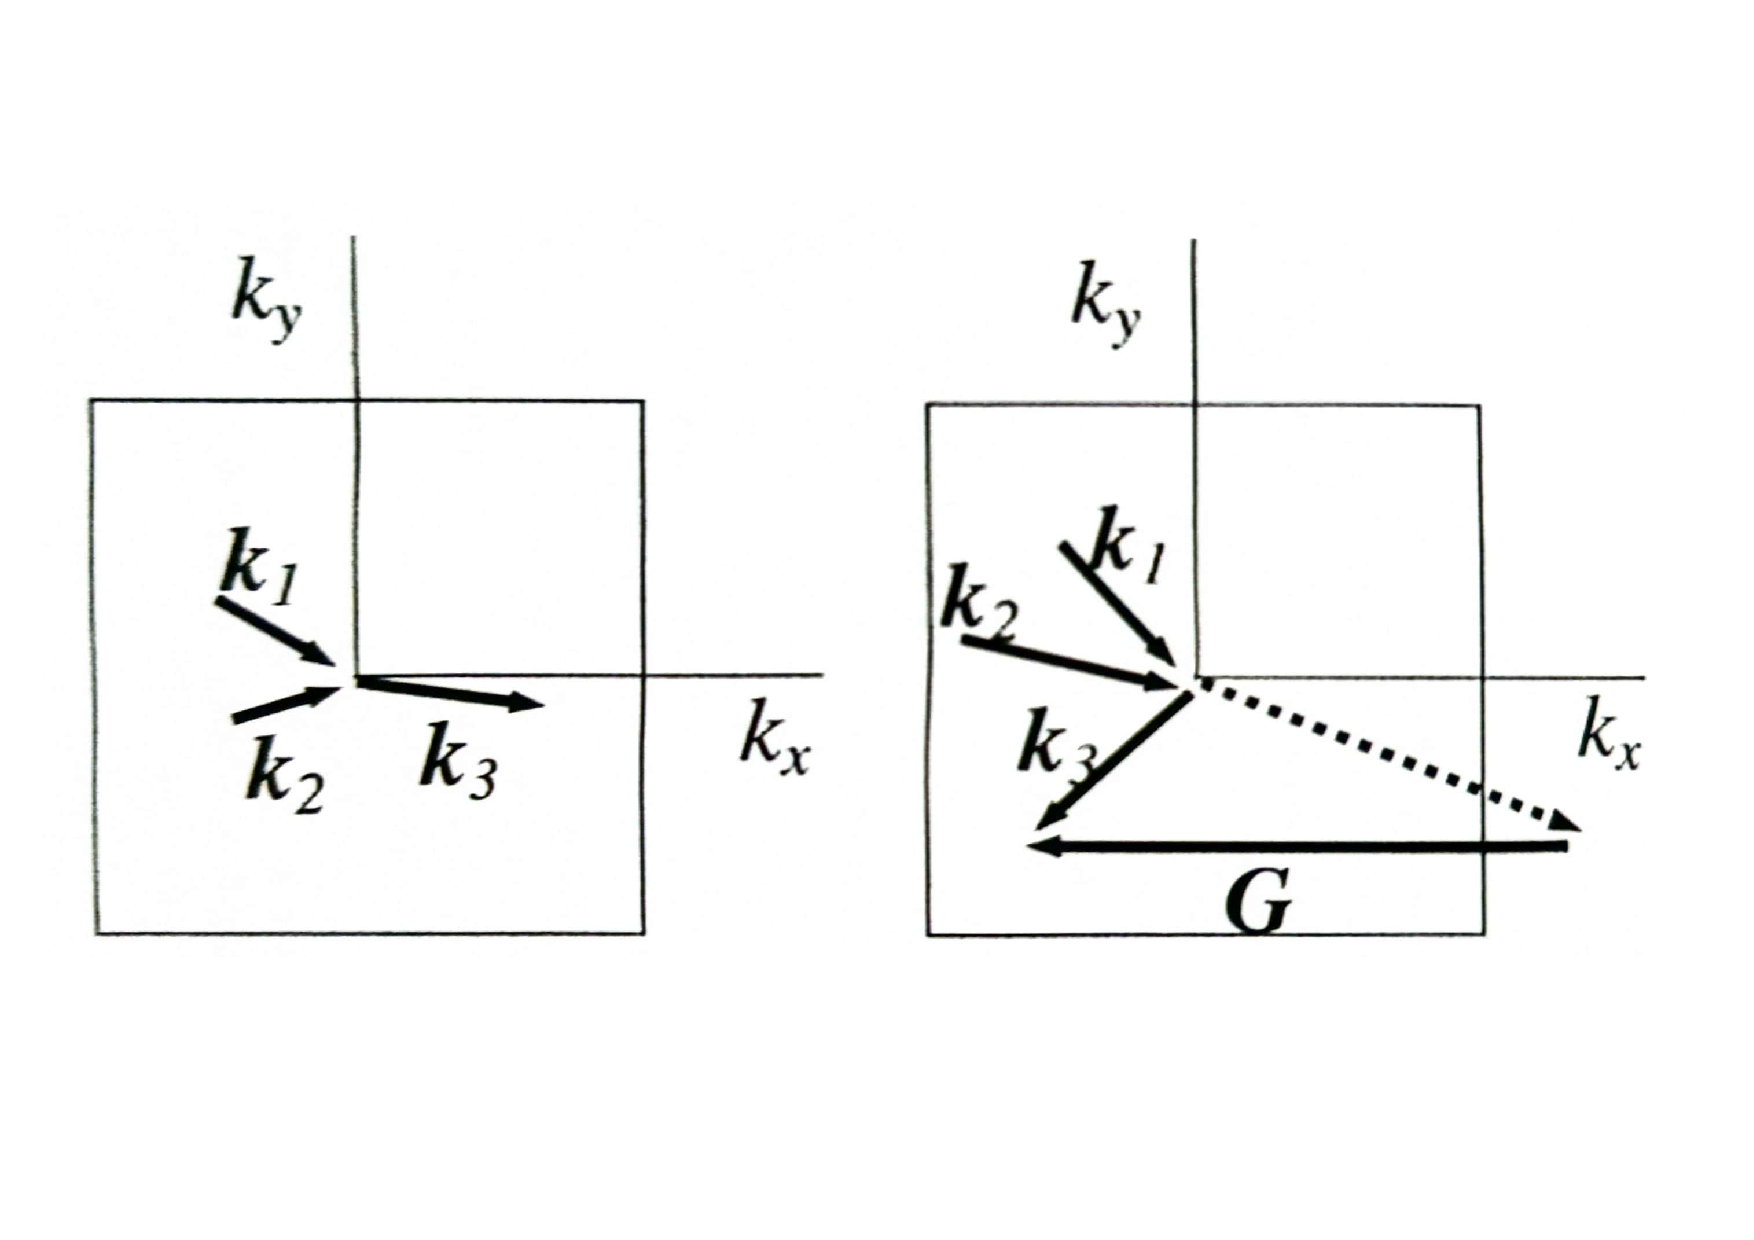
\includegraphics[scale=0.35]{Cuerpo/Ch_05/Fotos libro 8.pdf}
    \caption{Izquierda: Proceso $N$ que no degrada el transporte de energía térmica. Derecha: Proceso $U$ que degrada fuertemente el transporte de calor.}
    \label{Fig:05-08}
\end{figure}    

\subsubsection{Evolución de $\kappa$ con la temperatura}

A bajas temperaturas ($T\ll \theta_D$) el recorrido libre medio lo fija la calidad del cristal ya que no hay fonones con la suficiente energía para sufrir procesos $U$. Como $c_V \propto T^3$ resulta $\kappa \propto T^3$. Al aumentar la temperatura (aunque todavía a $T\ll \theta_D$) el número medio de fonones capaces de sufrir procesos $U$ serán aquellos con $\omega\approx\omega_D$, esto es, $\langle n\rangle_U \approx e^{-\theta_D / T}$. Admitiendo qeu $l\propto \langle n \rangle_U^{-1}$ se tendrá que $\kappa \propto T^3 e^{\theta_D/T}$. 

Cuando $T>\theta_D$ una proporción sustancial de todas las colisiones entre fonones serán procesos $U$. Entonces $\langle n \rangle_U \approx \langle n \rangle \approx k_B T / \hbar \omega$, con lo cual $l \propto T^{-1}$. Como estas temperaturas $c_V\approx$cte., se tiene $\kappa \propto T^{-1}$. La evolución global es, cualitativamente, la que ilustra en la figura \ref{Fig:05-09} (a). Como puede verse en la figura \ref{Fig:05-09} (b), está en buen acuerdo con la observación experimental en el caso de sólidos cristalinos.

\begin{figure}[h!] \centering
    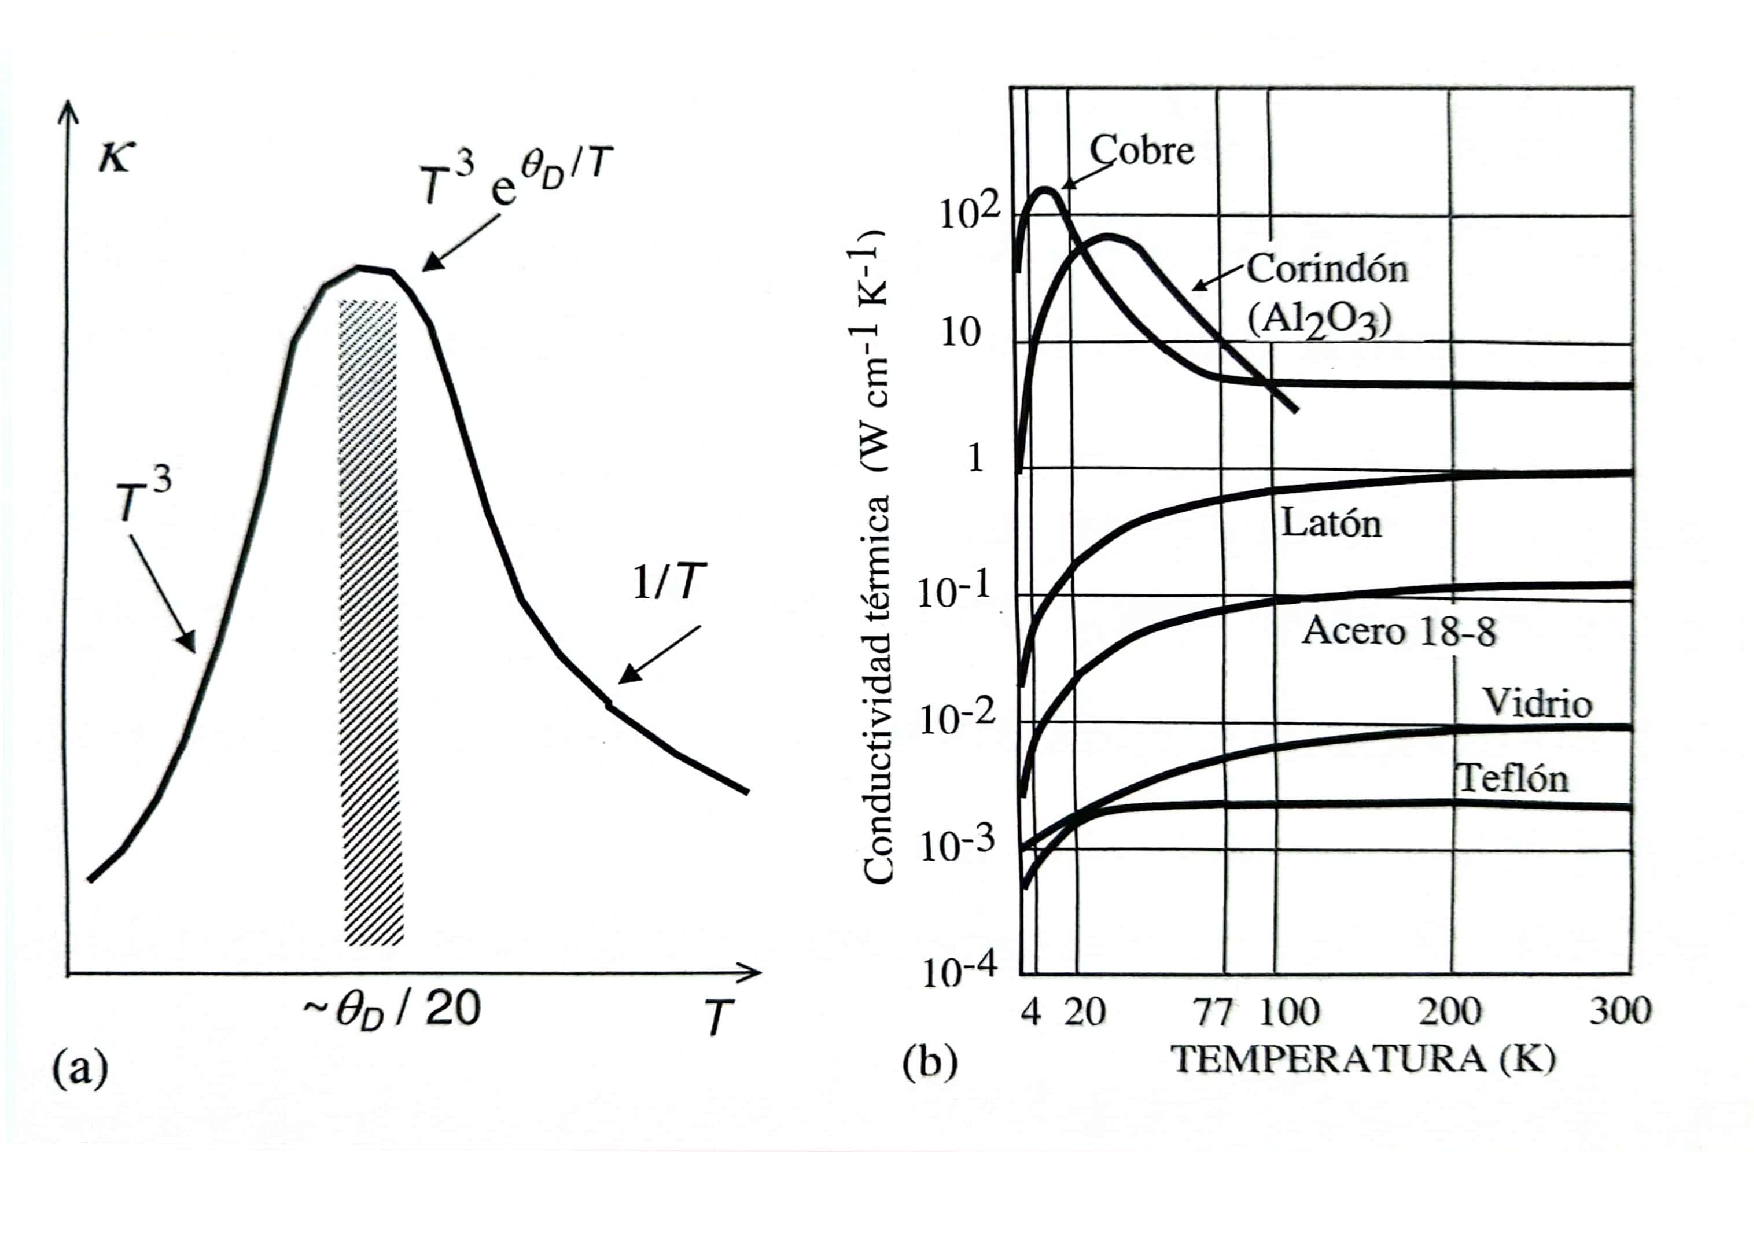
\includegraphics[scale=0.35]{Cuerpo/Ch_05/Fotos libro 9.pdf}
    \caption{(a) Dependencia genérica de la conductividad térmica de los cristales con la temperatura. (b) Conductividad térmica frente a la temperatura para diversos tipos de sólidos.}
    \label{Fig:05-09}
\end{figure}    

